\documentclass[aspectratio=169,10pt]{beamer}
\usepackage{common/pdmtheme}
\graphicspath{{figures/}}
\title[Pi 5 gateway]{Raspberry Pi 5 + AI HAT}
\subtitle{The gateway tier --- measured, and two assumptions refuted}
\author{Predictive Maintenance Platform}
\date{14 October 2026}
\begin{document}

\begin{frame}[plain]
  \vspace{5mm}
  {\LARGE\bfseries Raspberry Pi 5 + AI HAT (Hailo-8L)}\\[2mm]
  {\large\color{pdmink2} The gateway tier --- measured, and two assumptions
   refuted}\par
  \vspace{5mm}\noindent{\color{pdmrule}\rule{\linewidth}{0.4pt}}\par
  \vspace{3mm}
  \begin{columns}[T]
    \begin{column}{0.46\textwidth}
      \scriptsize
      \kv{Compute}{4$\times$ Cortex-A76 2.4 GHz, 8 GB}\\[1mm]
      \kv{Accelerator}{Hailo-8L, 13 TOPS}\\[1mm]
      \kv{Power}{7.5 W sustained, mains}\\[1mm]
      \kv{Score a frame}{\textbf{17 $\mu$s measured}}\\[1mm]
      \kv{Fan-out}{\textbf{781\,331 hourly nodes on one core}}\\[1mm]
      \kv{Cost}{$\sim$EUR 200 and it carries a site}
    \end{column}
    \begin{column}{0.46\textwidth}
      \scriptsize\color{pdmink2}
      The only figures in this repository from a \textbf{stopwatch} rather than
      a cycle count --- the gateway tier runs on general-purpose aarch64 Linux,
      and so did the measurement.
      \\[2mm]
      It was not a Pi 5. The benchmark says so in its own output and stores the
      caveat in its JSON, because a throughput number without its machine is
      unquotable.
    \end{column}
  \end{columns}
  \srcnote{Branch \texttt{hw/rpi5-hailo-gateway}. 18 gateway tests, 36 shared
  edge-agent tests. Figures generated from
  \nolinkurl{results/benchmark.json} and \nolinkurl{results/holdover.json}.}
\end{frame}

% ---------------------------------------------------------------- measured ---
\begin{frame}{What a gateway actually costs, measured}
  \centering
  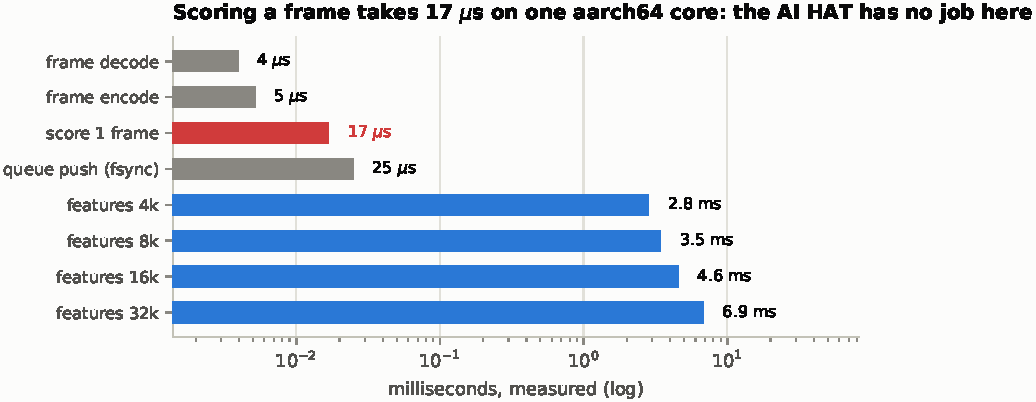
\includegraphics[width=0.78\textwidth]{rpi5_latency.pdf}
  \\[2mm]
  \begin{columns}[T]
    \begin{column}{0.49\textwidth}
      \scriptsize
      Five orders of magnitude, and the two stages an accelerator could touch
      are at the bottom of it. Scoring is \textbf{17 $\mu$s}; the feature
      extractor is 200$\times$ that; the acquisition it serves is 100$\times$
      the extractor.
    \end{column}
    \begin{column}{0.49\textwidth}
      \scriptsize\color{pdmcrit}
      \textbf{A measurement that measured nothing, and says so.}
      \par\color{pdmink2}
      The durable queue reported 39\,828 frames/s with
      \texttt{synchronous=FULL} --- implausible. The benchmark detects that
      \texttt{durable} and \texttt{nosync} agree within 20 \% and warns that the
      \texttt{fsync} is not reaching storage on this host.
      \\[1mm]
      A benchmark that silently measures nothing is worse than none, because
      the number gets quoted.
    \end{column}
  \end{columns}
\end{frame}

\begin{frame}{Refuted assumption 1: compute is not the constraint}
  \centering
  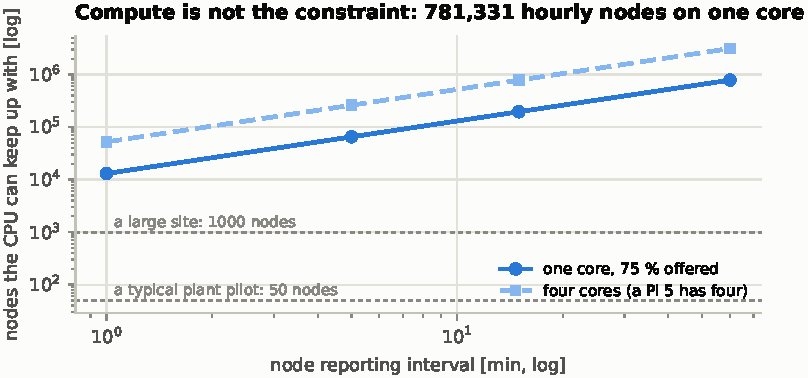
\includegraphics[width=0.72\textwidth]{rpi5_fanout.pdf}
  \\[1mm]
  \begin{columns}[T]
    \begin{column}{0.49\textwidth}
      \scriptsize
      One core, 75 \% offered, keeps up with \textbf{781\,331} hourly nodes. A
      large site has a thousand. Three orders of magnitude of headroom.
      \\[2mm]
      If compute were the reason for a gateway tier, a gateway tier would not
      be needed.
    \end{column}
    \begin{column}{0.49\textwidth}
      \scriptsize\color{pdmink2}
      What \emph{does} bind a gateway --- none of which this benchmark
      measures:
      \\[1mm]
      the broker's concurrent connections and memory per connection $\cdot$ the
      time-series database's write rate $\cdot$ the uplink $\cdot$ and
      \textbf{BLE airtime}, a shared medium with a hundred nodes waking on
      their own schedules.
      \\[1mm]
      Measuring them needs the compose stack running, and there is no Docker in
      this environment.
    \end{column}
  \end{columns}
  \takeaway{The accelerator is never the answer for feature-vector scoring ---
  the same conclusion the Alif branch reached on different silicon.}
\end{frame}

% -------------------------------------------------------------- the real job --
\begin{frame}{So what is a gateway for?}
  \begin{columns}[T]
    \begin{column}{0.47\textwidth}
      \scriptsize
      \textbf{1. Protocol translation.} A BLE node cannot reach a cloud
      broker, and the thing that terminates the radio is the only
      mains-powered element in the chain anyway.
      \\[1.5mm]
      \textbf{2. Site-scale store-and-forward.} A node's flash holds days; a
      gateway's SSD holds months.
      \\[1.5mm]
      \textbf{3. Local autonomy.} An alarm needing a cloud round trip is
      unavailable during the outage that most often \emph{accompanies} a real
      failure. The gateway scores locally and alarms with no uplink at all.
      \\[1.5mm]
      \textbf{4. Knowing which nodes have gone quiet.}
    \end{column}
    \begin{column}{0.47\textwidth}
      \scriptsize
      \textbf{(4) is the one that cannot live anywhere else.}
      \\[1mm]
      A node that stops reporting is the commonest real event in a deployed
      fleet, and downstream it is \textbf{indistinguishable from a healthy
      quiet machine} --- both produce no data. Only the thing the nodes report
      \emph{to} knows the difference.
      \\[2mm]
      \color{pdmink2}
      Three decisions, each with a failure behind it:
      \begin{itemize}\itemsep1pt
        \item interval \textbf{learned}, not configured --- fleet config drifts;
        \item learned \textbf{slowly} (EWMA 0.8/0.2) --- one early frame must
              not raise the threshold and mask the outage that follows;
        \item \textbf{three} missed intervals, not one --- crying wolf trains
              the operator to ignore it.
      \end{itemize}
      And silence is measured from \textbf{arrival}, not the frame's
      timestamp: a node with a wrong clock would look permanently fresh.
    \end{column}
  \end{columns}
\end{frame}

% ---------------------------------------------------------------- holdover ---
\begin{frame}{Refuted assumption 2: holdover is not the correctness requirement}
  \centering
  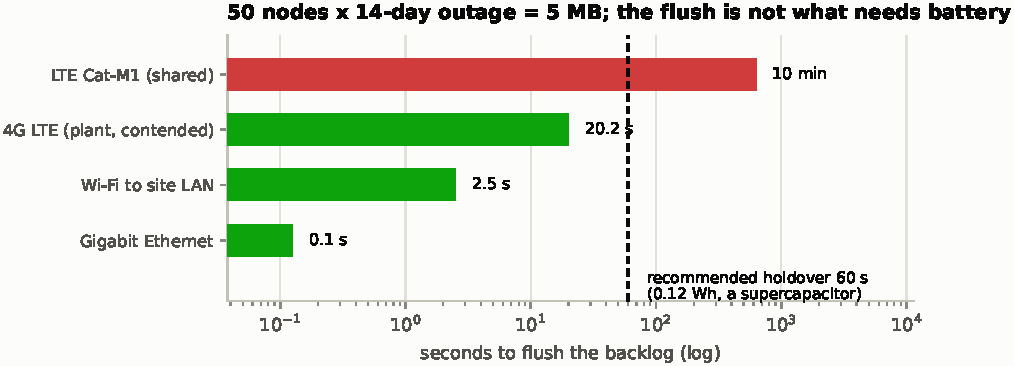
\includegraphics[width=0.80\textwidth]{rpi5_holdover.pdf}
  \\[2mm]
  \begin{columns}[T]
    \begin{column}{0.49\textwidth}
      \scriptsize
      This kit's own plan said ``UPS holdover is a correctness requirement''.
      It is not. The backlog is already safe --- SQLite
      \texttt{synchronous=FULL} fsyncs every frame --- and the flush happens
      when mains \emph{and} uplink are back, not on battery.
      \\[2mm]
      So the UPS buys a graceful SQLite close (30 s is generous) and
      brownout ride-through. \textbf{60 s of supercapacitor, 0.12 Wh} --- no
      battery chemistry in the enclosure, no maintenance item.
    \end{column}
    \begin{column}{0.49\textwidth}
      \scriptsize\color{pdmcrit}
      \textbf{The correction that matters more: storage.}
      \par\color{pdmink2}
      If the SD card dies on an unclean power-down, the site's backlog is gone
      whatever the holdover. An NVMe SSD or eMMC carrier is a larger
      data-integrity win \emph{and} costs less than the UPS it partly replaces.
      \\[2mm]
      The queue fsyncs once per frame: 1\,200 writes/day at 50 nodes hourly is
      trivial; 1 Hz aggregation across a large site would consume an SD card in
      months.
    \end{column}
  \end{columns}
\end{frame}

% ------------------------------------------------------------------ the HAT ---
\begin{frame}{The AI HAT: what it would take to earn its place}
  \centering
  \scriptsize
  \begin{tabular}{@{}lr@{}}
    \toprule
    & \textbf{Latency} \\
    \midrule
    63-float detector, numpy on one CPU core            & \textbf{17 $\mu$s} \\
    1D CNN over 8192 raw samples, $\sim$4 MMAC, on CPU  & $\sim$8 ms \\
    the same CNN on a Hailo-8L                          & $\sim$0.3 ms \\
    \quad \ldots for 200 channels at once               & still $\sim$0.3 ms \\
    \bottomrule
  \end{tabular}
  \\[3mm]
  \begin{columns}[T]
    \begin{column}{0.48\textwidth}
      \scriptsize
      The HAT is justified by a \textbf{model class}, not a speed-up: a raw
      waveform model skips the feature extractor entirely.
      \\[1mm]
      That is the appeal --- every feature here is a human decision about what
      matters, taken in advance --- and the risk: a waveform model can learn
      the test rig's mains hum and call it a bearing fault.
    \end{column}
    \begin{column}{0.48\textwidth}
      \scriptsize
      \textbf{\texttt{HailoScorer} raises on construction}, and the exception
      lists what is missing:
      \begin{enumerate}\itemsep0.5pt
        \item a 1D CNN trained on \emph{measured} data;
        \item ONNX $\rightarrow$ \texttt{.hef}, int8-calibrated on real
              waveforms;
        \item a bit-exactness check against the ONNX reference;
        \item decision-flip accounting against the float model.
      \end{enumerate}
      \color{pdmcrit}
      A stub returning plausible probabilities would make this kit look
      finished while shipping confident scores from a nonexistent model.
    \end{column}
  \end{columns}
  \takeaway{Buy the Pi, skip the HAT, spend the EUR 70 on the NVMe SSD ---
  where it buys data integrity.}
\end{frame}

% ------------------------------------------------------------------ status ---
\begin{frame}{Status, and what is deliberately absent}
  \begin{columns}[T]
    \begin{column}{0.50\textwidth}
      \scriptsize
      \begin{tabular}{@{}ll@{}}
        \toprule
        Fan-in, forwarding, queueing      & 18 tests \\
        Gap detection, wrap-safe          & \checkmark \\
        Local alarms during an outage     & \checkmark \\
        Silent nodes, learned intervals   & \checkmark \\
        Corrupt frame rejected            & \checkmark \\
        Bad scorer does not stop forwarding & \checkmark \\
        Throughput measured               & this host \\
        \midrule
        Run on a Pi 5                     & \textcolor{pdmcrit}{no} \\
        \texttt{fsync} cost measured      & \textcolor{pdmcrit}{no} \\
        Compose stack started             & \textcolor{pdmcrit}{no} \\
        Hailo-8L used                     & \textcolor{pdmcrit}{by design, no} \\
        Radio termination                 & not written \\
        \bottomrule
      \end{tabular}
    \end{column}
    \begin{column}{0.46\textwidth}
      \scriptsize
      \textbf{The radio side does not exist, deliberately.}
      \texttt{Gateway.handle()} takes bytes. What delivers them --- a BLE GATT
      server, a sub-GHz concentrator, a local broker --- is the one part that
      genuinely depends on the radio hardware chosen, and stubbing it would
      hide the choice.
      \\[2mm]
      \color{pdmink2}
      \textbf{The undecided question a review should force:} may the gateway
      read node payloads? If it can, compromising one gateway compromises a
      site. If it cannot, local scoring --- reason (3) for having a gateway at
      all --- stops working. That trade should be decided deliberately, and it
      has not been.
    \end{column}
  \end{columns}
\end{frame}

\end{document}
